\chapter{Background}\label{chap:background}

\hl{
This work builds upon prior work on WCA applications, and it leverages
existing work in computer vision.
}
This chapter provides an overview of this work in addition to a comparison
between WCA and other computerized aids for assembly tasks.

\section{Aids for Assembly Tasks}

\hl{
  We consider three types of people who are involved with WCA applications.
  The first are \emph{users}, who are completing a task and receiving guidance
  from the application.
  The next are \emph{experts}, who are familiar with the tasks, and the mistakes
  that a user might make.
  Some systems (including ours) allow experts to help users with a task, over a
  video call.
  The last type of people are \emph{developers} who create a WCA application for
  a specific task, but developers are not involved at the point that a user
  is completing the task.
}

\hl{
  A large body of work has been done by other researchers on systems to aid with
  assembly tasks.
}
However, none of these systems determined when steps were completed using
computer vision models that processed data from an RGB camera.
\hl{
In contrast to some previous work, the techniques we
propose do not require instrumenting parts of workspaces with sensors.
}
Our system also does not require the person who is completing the task to
determine when a step has been completed, and then indicate this to the system.
\hl{
  In addition, our system does not require the continuous attention of a task
  expert to observe a user for the entire duration of that task.
  The application starts out providing automated guidance, and only starts a call
  with a task expert when the user requests help from a human.
}
This burdens task experts much less than a system where the task expert must be
on a call to help a user with the full task.

\citet{webuild} developed a system to distribute steps for an assembly task
among members of a group completing the task together. Instructions are
displayed on a smartphone screen, and users manually press a
button to indicate when a step is completed.
Their system has no way to automatically detect when a step is completed, and
it does not handle user errors.
The authors ran a user study where people assembled an IKEA cabinet and a
Meccano bridge kit.
Requiring people completing the task to indicate when a step is completed
creates an additional burden that our system avoids.
\citet{sensors} developed a system that
determines when steps for assembling an Ikea wardrobe have been completed, using
sensors such as gyroscopes, accelerometers, force sensing resistors, and
infrared distance meters. This system allows users to complete steps of the task
in different orders.
However, their system was purely focused on detecting completed steps, and it
did not give the users any instructions.
\citet{kinect} used a Kinect
sensor to guide users through assembling objects out of Duplo blocks. The system
determined when steps were completed by processing data from the Kinect sensor.
Duplo blocks have bright colors and simpler shapes than the objects that our
tasks use.
\citet{smartwatch} developed a system that provides instructions to users on
smartwatch displays, and determines when steps have been completed using sensors
that are typically present in a factory environment, such as RFIDs and infrared
light barriers~\cite{smartwatch2}.
Our system does not require the presence of such sensors.

\citet{robotic_arm}'s system guided users through assembling a pavilion out of
bamboo sticks. The users moved around a room, picking up certain sticks and
then delivering them to a robotic arm. Users wore Apple Watches, and were given
written instructions on the watches' displays. A user swiped on the face to see
the next instruction. The locations of each user were also tracked using BLE
beacons that communicated with iPhones that users carried. A centralized system
used the location information to decide the next instruction that should be
given to each user.
This system requires users to manually request the next instruction, while our
system automatically gives the next instruction after the user completes a step.

\citet{collaboration} examined systems where remote experts helped users with
assembly tasks. The people completing tasks communicated using a tablet for one
task, and a Google Glass for another. In addition,
they looked at a case where where the user could stay in one place and a case
where the user had to move across different workspaces to complete the task.

Table~\ref{table:prior_work} provides a brief summary of all of the existing
systems described in this section.

\begin{table*}
  \begin{tabular}{| l | p{2in} | p{2.5in} |}
    \hline
    Prior Work & Detection of Step Completion & Other Attributes\\
    \hline
    \citet{webuild} & User presses a button & Multiple users working on task
                                              together.\\
    \hline
    \citet{sensors} & Automatic, using gyroscopes, accelerometers, force sensing
                      resistors, and more & Requires sensors to be installed in
                                            the Ikea parts. Did not give
                                            instructions.\\
    \hline
    \citet{kinect} & Automatic, using Microsoft Kinect & Builds a full virtual
                                                         model of what the user
                                                         has constructed. Only
                                                         supports large colorful
                                                         duplo blocks. \\
    \hline
    \citet{smartwatch} & Automatic, using RFIDs and infrared light barriers
                                              & Requires sensors to be present
                                                in working environment.\\
    \hline
    \citet{robotic_arm} & Manually from user
                                              & The final assembled object was
                                                massive. Many parts were
                                                identical.\\
    \hline
    \citet{collaboration} & Remote task expert
                                              & Compared Tablet with Google
                                                Glass.\\
    \hline
\end{tabular}
\caption{
  Existing systems that helped users with physical assembly tasks.
}\label{table:prior_work}
\end{table*}

\section{Wearable Cognitive Assistance}

\begin{table*}[h!]
\begin{tabular}{|p{0.40in}|p{1in}|p{3.2in}|p{0.7in}|p{0.8in}|}
\hline
App Name & Example Input Video Frame & Description & Symbolic Representation & Example Guidance \\
\hline
\textbf{Pool} & \raisebox{-0.9\totalheight}{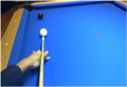
\includegraphics[width=0.97in]{figures/table_existing/example-pool.png}}
&
Helps a novice pool player aim correctly. Gives continuous visual feedback (left arrow, right arrow, or thumbs up) as the user turns his cue stick.  The symbolic representation describes the positions of the balls, target pocket, and the top and bottom of cue stick.
&
$<$Pocket, object ball, cue ball, cue top, cue bottom$>$ &  \raisebox{-0.85\totalheight}{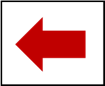
\includegraphics[width=0.8in]{figures/table_existing/guidance-pool.png}} \\
\hline
 \textbf{Ping-pong} & \raisebox{-0.9\totalheight}{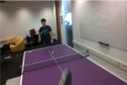
\includegraphics[width=0.97in]{figures/table_existing/example-pingpong.png}}
&
Tells novice to hit ball to the left or right, depending on which is more likely to beat opponent. Uses color, line and optical-flow based motion detection to detect ball, table, and opponent.
&
 $<$InRally, ball position, opponent position$>$ & ``Left!'' \\
\hline
 \textbf{Work-out} & \raisebox{-0.9\totalheight}{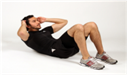
\includegraphics[width=0.97in]{figures/table_existing/example-workout.png}}
&
Counts out repetitions in physical exercises. Classification is done
using Volumetric Template Matching on a 10-15 frame video segment.  A
poorly-performed repetition is classified as a distinct type of
exercise (e.g. ``good pushup'' versus ``bad pushup'').
&
 $<$Action, count$>$ & ``8'' \\
\hline
 \textbf{Face}     & \raisebox{-0.9\totalheight}{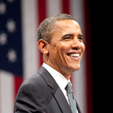
\includegraphics[width=0.8in]{figures/table_existing/example-face.png}}
&
Jogs your memory on a familiar face whose name you cannot recall. Detects and extracts a tightly-cropped image of each face, and then applies a state-of-art face recognizer. Whispers the name of the person recognized.
&
 ASCII text of name & ``Barack Obama'' \\
\hline
 \textbf{Lego} & \raisebox{-0.9\totalheight}{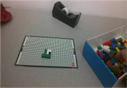
\includegraphics[width=0.9in]{figures/table_existing/example-lego.png}}
&
Guides a user in assembling 2D Lego models.  The symbolic representation is a matrix representing color for each brick.
                                                   &
{\small [[0, 2, 1, 1], \break [0, 2, 1, 6], \break [2, 2, 2, 2]]} & ``Put a 1x3 green piece on top'' \\
\hline
 \textbf{Draw} & \raisebox{-0.9\totalheight}{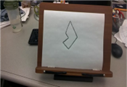
\includegraphics[width=0.9in]{figures/table_existing/example-draw.png}}
&
Helps a user to sketch better. Builds on third-party app for desktops. Our implementation preserves the back-end logic. A Glass-based front-end allows a user to use any drawing surface and instrument. Displays the error alignment in sketch on Glass.
&
\raisebox{-0.85\totalheight}{
\includegraphics[width=0.7in]{figures/table_existing/symbolic-draw.png}} & \raisebox{-0.95\totalheight}{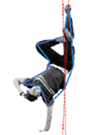
\includegraphics[width=0.7in]{figures/table_existing/guidance-draw.png}} \\
\hline
 \textbf{Sand-wich} & \raisebox{-0.9\totalheight}{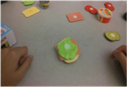
\includegraphics[width=0.97in]{figures/table_existing/example-sandwich.png}}
&
Helps a cooking novice prepare sandwiches according to a recipe. Since real food is perishable, we use a food toy with plastic ingredients. Object detection uses Faster-RCNN deep neural net approach.~\cite{frcnn}
&
 Object: \break ``E.g. Lettuce on top of ham and bread'' & ``Put a piece of bread on the lettuce'' \\
\hline

\end{tabular}
\caption{Example Wearable Cognitive Assistance Applications. The input frame is
  sent to a cloudlet, which converts it to the symbolic representation. The
  symbolic representation is then used to give guidance.
  (Source: Adapted from Satyanarayanan~\cite{Satya2017})
}\label{table:existing_wca}
\end{table*}

A WCA application provides just-in-time guidance and error detection for a user
who is performing an unfamiliar task.
Prompt error detection is also valuable for a user who is performing familiar
tasks, since human errors cannot be completely avoided, especially when the user
is tired or stressed.
Informally, WCA is like having ``an angel on your shoulder.''~\cite{ha2014}
It broadens, the metaphor of GPS navigation tools that
provide real-time step-by-step guidance, with prompt error detection and
correction.

This thesis builds on top of past research on WCA applications.
\citet{ha2014} introduced the first version of a programming framework called
Gabriel.
This framework includes networking and runtime components for WCA applications.
\citet{chen2017} developed an initial set of WCA applications, determined
how much latency was acceptable for these applications, and examined how changes
to the network, hardware, and algorithms used can affect end to end latency.
\citet{wang2019} examined how to reduce  the load imposed
on a cloudlet by a single WCA user, thereby allowing many more
users to share single cloudlet.
\citet{pham2021ajalon} developed a toolchain that
allows people to develop WCA applications without writing any code.

\hl{
 Table~{\ref{table:existing_wca}} lists some examples of WCA applications that
have developed in prior work.
In total, those researchers have developed over 15 WCA applications.
This work focuses on applications that that help users assemble physical
objects.}
\citet{chen2017} \hl{developed such applications for an IKEA lamp, a Lego kit,
and a toy sandwich.
We developed applications for an IKEA cart, a model car, a smartphone sanitizer,
a model plane, a Meccano bike it, and a Stirling engine.
}

These applications are a compelling use case for edge computing.
They first capture images using the camera on a mobile device, such as a
smartphone or head-mounted wearable device.
The images are then sent to a cloudlet for processing, using the Gabriel
platform~\cite{ha2014}.
\hl{
The computational limitations of lightweight mobile devices that have acceptable
battery life prevent applications from processing images using the
devices' own hardware~{\cite{Satya2009}}.
}
Table~\ref{fig:wca_apps} lists the resource consumption and end-to-end latency
bounds of five offloading-based WCA applications.
It shows that WCA applications are simultaneously compute-intensive,
bandwidth-hungry, and latency-sensitive.

\begin{table*}
    \begin{tabular}{|l||c|c|c|c|c|}
    \hline
    & Pool & Ping-pong & Face & Lego & Sandwich \\
    \hline
    \hline
    Cloudlet CPU load(\%) & 72.10 & 45.40 & 75.60 & 52.20 & 85.10 \\
    \hline
    End-to-end latency bounds (tight--loose, ms)* & 95--105 & 150--230 & 370--1000 & \multicolumn{2}{c|}{600--2700} \\
    \hline
    Video streaming bandwidth requirement    & \multicolumn{5}{c|}{480p:~~ 3.6 / 7.0} \\
    ~~~~~(Average / Peak, Mbps)              & \multicolumn{5}{c|}{720p:~~ 6.8 / 9.9} \\
                                             & \multicolumn{5}{c|}{1080p:~~ 8.1 / 12.7} \\
    \hline
    \end{tabular}
    \caption{
      CPU load, latency bounds, and the required bandwidth of example WCA
      applications.
      The implementations of the application servers~\cite{chen2017} were tested
      on a laptop (with an Intel$^{\mbox{\footnotesize\textregistered}}$
      Core$^{\mbox{\footnotesize\texttrademark}}$ i7-8500Y processor and 8GB RAM),
      running the frontend on an Android phone, using 480p, 720p, and 1080p
      video resolutions.
      (*) End-to-end latency includes both the round trip time (RTT) from the
      Android phone to the cloudlet and compute time in the cloudlet.
      Tight and loose bounds are adopted from Chen, et al,~\cite{chen2017}
      where they are defined:
      ``The tight bound represents an ideal target, below which the user is
      insensitive to improvements. Above the loose bound, the user becomes aware
      of slowness, and user experience and performance is significantly
      impacted.''
    }\label{fig:wca_apps}
\end{table*}

Our work extends this body of research in the following ways:
\begin{itemize}
\item Utilizing new computer vision techniques to support more realistic
  assembly tasks.
\item Adding live call support to WCA applications, so human experts can help
  users correct errors they make with tasks.
\item Training computer vision models using synthetic training images.
\item Developing a new software framework for WCA applications, that allows
  multiple users to share a single instance of an application running on a
  cloudlet.
\item Exploring how well DNNs running on mobile device hardware can support
  WCA applications.
\end{itemize}

\section{Computer Vision}

This work's contribution is in how computer vision (CV) is being applied, rather
than developing any new CV algorithms.
\hl{
  This section highlights the CV research that we leverage in our work.
}

\hl{
  We follow the lead of} \citet{gebru2017finegrained}, \hl{who used a two step
  process to find and distinguish cars that appeared in Google Street view
  images.
}
  Their first step was finding the
regions of images that were likely to contain cars. Then their second step was
classifying the type of car in that region.
\hl{
  We leverage their approach to train models on our own new
  data using existing neural architectures.
}

Image classifiers give a single class label for a full image, and do not provide
a bounding box. These are most useful when a scene has already been cropped to a
region involving a single object. Imagenet~\cite{ImageNet_VSS09} is a
classification dataset which contains classes for 1000 objects. Object
detectors provide bounding boxes and labels for objects in an image. This is
particularly helpful
when an object might only take up part of the camera view, or there might be
multiple objects visible
at once. Microsoft COCO~\cite{coco} is an object detection dataset with 80
classes.
Faster R-CNN~\cite{frcnn} is an object detector that is used in our
lamp~\cite{lamp} and toy sandwich~\cite{sandwich} assembly assistants.

Imagenet has the classes ``race car,'' ``sports car,'' and ``streetcar,''
in addition to classes for objects that aren't cars.
The Stanford Cars dataset~\cite{KrauseStarkDengFei-Fei_3DRR2013} is more
fine-grained, with images of cars that are labeled with the year, make, and
model.
\hl{
  The fine-grained dataset requires classifying cars based on small intricate
  details, while classifying cars into the three coarse-grained categories is
  simpler.
  This increase in complexity is similar to the increase in complexity between
  the work of} \citet{chen2017} \hl{and the work presented in this dissertation.
}
The Fast MPN-COV~\cite{Li_2018_CVPR} image classifier performs
well on several fine-grained classification datasets.

\hl{Our work is not the first to use object detection models for tasks beyond
detecting the objects in an image and providing their coordinates.}
Object detectors have been used for finding screws in pictures of aircraft
parts~\cite{visapp19} and consumer electronics~\cite{FOO2021666}.
\citet{wu2018spot} found differences between book covers using a modified
version of Faster R-CNN.

\section{Synthetic Training Data}

Training CV models in order to develop a WCA application for a specific task
requires thousands of labeled images.
Collecting and labeling this data requires a substantial effort, and it must be
repeated for each new WCA application.
\hl{Training models with synthetic data would eliminate or reduce the need for
  WCA application developers to collect and label real images.}

The idea of avoiding manual labeling has a long and rich history.
\citet{synthetic} trained an object detector on synthetic data that
outperformed an object detector trained on real data. They generated backgrounds
cluttered with distractor objects. In addition, they added some distractor
objects to the foreground and varied the lighting conditions that were used to
render each of the images. These images looked 3D, but they were not
photo-realistic. Other works have generated photo-realistic images to use as
training data~\cite{DBLP:journals/corr/abs-1809-10790, photo2}, or used real
background images~\cite{real_background1, real_background2, real_background3}.
\citet{dwibedi} avoided rendering 3D graphics altogether by cropping objects
from photographs, and pasting these crops into other photographs.
Their models trained on synthetic images performed worse than their models
trained on real images.
However, they also  trained models using a mix of real and synthetic images, and
these performed better than models trained on real or synthetic data alone.

\section{Hierarchical Decomposition}

\citet{Simon1991} argued that all complex systems are made up of smaller
systems. These smaller systems are made up of even smaller systems, thus
forming a hierarchy with several layers.
Reasoning about a smaller system on its own is easier than trying to understand
a full system all at once.
We can apply this idea to state detection for WCA applications by decomposing
a large assembly task into separate smaller sub-assemblies.
This limits the scope of what any one computer vision model that we use is
responsible for.
It also allows multiple developers to work on computer vision models for
different parts of the task completely independently from each other.
Finally, it also simplifies performance of a task over an extended period
(e.g. multiple days). A person who has to stop work in the middle of a task will
have an easier time if the task is split into subtasks that don't require any
context from earlier subtasks. They can start work from the beginning of a
subtask every time, rather than having to recall anything about steps they
completed the last they they worked on the task.

\citet{semantic_hierarchy} utilized hierarchies of visual features to recognize
objects.
\citet{subassembly_identification} automatically identified subassemblies of
assembled objects based on CAD files.
They utilize features such as the number of other parts that a certain part
touches, or the amount of surface area that two touching parts share.
They considered subassemblies from the perspective of assembly sequence
planning, rather than detecting completed task steps using computer vision.

\section{Development Toolchain}

\citet{pham2021ajalon}
\hl{
  created a set of tools called Ajalon, that developers can use to create WCA
  applications for assembly tasks.
  They utilized Intel's Computer Vision Annotation Tool (CVAT)~{\cite{CVAT}} and
  developed Open Workflow Editor~{\cite{workflow}}, a state machine editor.
  The authors ran a user study with developers to show that their toolchain is
  effective.
}